\documentclass[UTF8, 11pt, a4paper]{ctexart}
\usepackage{geometry}                		% See geometry.pdf to learn the layout options. There are lots.
\geometry{a4paper} 
%\geometry{landscape}                		% Activate for rotated page geometry
%\usepackage[parfill]{parskip}    		% Activate to begin paragraphs with an empty line rather than an indent
\usepackage{graphicx}				% Use pdf, png, jpg, or eps§ with pdflatex; use eps in DVI mode
								% TeX will automatically convert eps --> pdf in pdflatex		
\usepackage{amssymb}
%% LaTeX - Article customise

%%% PACKAGES
\usepackage{booktabs} % for much better looking tables
\usepackage{array} % for better arrays (eg matrices) in maths
\usepackage{paralist} % very flexible & customisable lists (eg. enumerate/itemize, etc.)
\usepackage{verbatim} % adds environment for commenting out blocks of text & for better verbatim
\usepackage{subfigure} % make it possible to include more than one captioned figure/table in a single float
% These packages are all incorporated in the memoir class to one degree or another...

%%% ToC APPEARANCE


\usepackage{graphicx,amssymb}
\usepackage{fontspec,xltxtra,xunicode}
\usepackage{caption,float,hyperref}
\usepackage{amsmath, amssymb}

%% END Article customise
%SetFonts
\setCJKmainfont[BoldFont=Songti SC Bold, ItalicFont=Songti SC]{Songti SC}
\setCJKsansfont[BoldFont=Songti SC Bold]{Songti SC}
\setCJKmonofont{Songti SC}

\setmainfont{Times New Roman}
\defaultfontfeatures{Mapping=tex-text}
\setromanfont[Mapping=tex-text]{Times New Roman}
\setsansfont[Scale=MatchLowercase,Mapping=tex-text]{Times New Roman}
\setmonofont[Scale=MatchLowercase]{Times New Roman}

%SetFonts
\hbadness=10000
\tolerance=10000
\hfuzz=150pt

\title{量子计算机运算存储体系
结构综述}
\author{陈思宇\texttt{sychen@zju.edu.cn}}
\date{\today}  

\begin{document}
\maketitle


\begin{abstract}
本文基于近几年计算机科学、计算机体系结构与量子计算、并行计算的发展,选取部分有亮点的文献材料,针对其中提出的概念、理论、观点与创新结构作以综述。希望借助此文,从细节与硬件层面、物理层面入手,展现量子计算一些小方面实实在在的进展成果。

\bf{关键字}: 计算机体系结构;量子计算;存储器;运算器
\end{abstract}

\newpage
\tableofcontents

\newpage
\section{概述}
量子计算作为一个前沿概念,代表着计算机体系结构的一个全新的设计空间与发展方向,量子计算机的特性使得其允许更多全新思路的计算机体系结构得以构想,甚至在未来得以实现。通常,在计算机领域,即使是不同研究方向的科研工作者,对彼此的研究内容也有一定基础型的了解,比如进行人工智能研究的研究者也有数据库领域的知识,并大都具有数据库、操作系统、芯片硬件、甚至前端后端工程领域的经验。

然而,量子计算的深艰概念与复杂的理论性使得一般的、广义的计算机科学研究领域与研究者对此大都并不甚知。相反地,这一类对计算机领域影响深远的学科常由物理、机械电子等科研机构深入研究,这使得量子计算这项前沿计算机技术在某种程度上与计算机科学隔绝。

在本文中,我们将列出一些关键的量子计算概念,并从务实的角度,介绍与叙述构成量子计算机体系结构的量子设施,并描述一些可以进行配合的先进方法,最后,提出一些领域存在的问题与领域的展望。

\newpage
\section{基于量子科学的体系结构原理}
\subsection{量子的基本物理概述}

从物理的角度,“量子”一词本身并不指代任何物质。“量子”所代表的是一种非连续化的性质,可以指代能量的非连续性、空间位置的非连续性,和自旋(spinning)、相位(phase)取值的非连续性,同时也指代这些性质之间的干涉(Interference)现象与纠缠(entanglement)、叠加(superposition)等现象。少数微观粒子在能量、位置、自旋、相位等方面表现出了量子性,比如电子、反电子和光子\cite{shortq},而由微观粒子组成的宏观粒子与物质却因为decoherence\cite{shortq}\cite{introq}而不能明显地展现这种特性。由此,我们称一些能够表现量子性的微观粒子为“量子粒子”,它们具有“量子性”,比如一个被束缚的带有1/2正自旋的电子,或一个封闭环境中带有1自旋的光子。

\subsection{量子架构下信息的可表达性}

对于普通的二进制电子计算机,借助激光刻蚀在单晶硅上行程的NP节中电平(电子)的有无,电子计算机得以保存信息的状态;借助能够对电平有无进行运算的逻辑门,电子计算机得以对信息进行计算。而对于量子粒子,只有其自旋状态可变,这也成为量子计算的唯一自由度\cite{shortq}。

一般来说,孤立的光子电子都只有一个量子数:极向;电子为轨道;亚粒子为自旋。但当粒子处于复杂环境中时,为了描述环境对它的影响,就要引入更多的变量。比如当电子环绕原子核时,受到强力干预而产生可观测的能级性质,并且收到核子磁效应而产生不同的行为,此时为了描述电子,泡利引入了4个量子数:主量子数$n$、角量子数$l$、总角量子数$j$、总磁量子数$m_{j}$\cite{shortq}。为了方便通用地描述量子粒子的特性,我们使用波函数形式来进行表示\cite{introq},如公式\ref{eq:wave}

\begin{eqnarray}
\label{eq:wave}
| \Psi \rangle & = & [c_{0},c_{1},c_{2},...,c_{n-1}]^{T} \\
\label{eq:eigenstate}
\| | \Psi \rangle \|&=&1\hspace{2pt}mod \hspace{2pt} 1
\end{eqnarray}

因为自旋可以有两种方向,所以可将一个电子的状态描述为:

\begin{equation}
| \Psi \rangle = c_{0} \cdot \left[\begin{array}{c}1 \\0\end{array}\right] + c_{1} \cdot \left[\begin{array}{c}0 \\1\end{array}\right]
\end{equation}

对于常见的内禀角动量,可以用一个复数来表示,这既能表示相位,也能表示转动量,因为复数复分量的物理含义就是逆时针旋转。

\begin{eqnarray}
| \Psi \rangle &=& \frac{(5+2i) \cdot |\uparrow\rangle + (-2+i) \cdot |\downarrow\rangle}{\sqrt{34}} \\
| \Psi \rangle &=& \frac{1}{\sqrt{34}} \left[\begin{array}{c}5+2i \\ -2+i \end{array} \right] 
\end{eqnarray}

上述数学式所描述的是两种自旋方向$|\uparrow\rangle$,$|\downarrow\rangle$ 共存的叠加态(superposition),这也是量子计算非常重要的特性—状态的同时性。

基于复变函数的薛定谔方程也都采用复数形式,并常常用模拟性的欧拉公式作以变换,如下式\ref{eq:euler}。

\begin{equation}
\label{eq:euler}
e^{{i\theta ({\hat  {{\mathbf  {n}}}}\cdot {\boldsymbol  {\sigma }})}}=I\cos \theta +i({\hat  {{\mathbf  {n}}}}\cdot {\boldsymbol  {\sigma }})\sin \theta \,
\end{equation}

根据式\ref{eq:euler},我们可以用一个通用的方法来表示量子态的等权重叠加,形式如\ref{eq:eulersuperpos}所示。

\begin{equation}
\label{eq:eulersuperpos}
|\Psi\rangle =  |\Psi_i\rangle \bigoplus |\Psi_j\rangle = \left[ e^{ikx_j}|\downarrow\rangle_i |\uparrow\rangle_j \pm e^{ikx_i}|\uparrow\rangle_i |\downarrow\rangle_j \right] / \sqrt{2}
\end{equation}

对于两个量子状态$c_1=5+3i ,c_2=-3-2i$,我们知道第一个状态对应的模是34,第二个是13,但是如果我们将两个复态加和则会出现$|c_1+c_2|^2=5<13<34$,此时两个状态的结合产生了一个小于两者其中任意一个的新状态,这种现象在物理过程中实际发生时,即可称为量子干涉。另外基于量子事件的概率数属于概率空间,考虑到量子操作的封闭性与可逆性,量子状态的迁移概率矩阵$M$必须是一个酉矩阵,也就是$U\cdot U^{\dagger}=I$其中$U^{\dagger}$表示矩阵的共轭转置。对于矩阵$|U[i,j]^2|$,其任意行或任意列的加和都是1(注意这里取模后$|i|^2$的数值变为1而不是-1)。对一个状态矩阵$U$来说,其共轭转置矩阵$U^\dagger$实际的物理含义经过运算观察,也比较容易理解,如果对一组状态施加$U$使其概率状态发生演进,那么也可以通过对其施加$U^\dagger$使其状态回退一步。从物理角度,这种可反演性是系统的信息封闭性与完备性的体现。

当遇到两个量子系统$A,B$,大小分别为$N_A,N_B$,两者组合时,新的状态迁移矩阵大小应为$N_C=N_A \times N_B$,新的状态矩阵原先两个状态矩阵的张量积,表示为$C=A\otimes B$。这个概念十分重要,因为在计算机的硬件实现中,每个量子位都是一个独立的系统,为了应对运算和存储的任务,我们不可避免地要将几十上百个量子粒子排排放,这些量子位所含状态的全体构成了一台量子计算机的表示空间,这个空间的大小与状态迁移都由坎氏积来定义。形式语言上,假设$| \psi \rangle$表示某一个系统,$| \psi ' \rangle$表示另一个系统,则有下式\ref{eq:phiadd}所示
\begin{equation}
\label{eq:phiadd}
| \psi \rangle \otimes | \psi ' \rangle = | \psi , \psi ' \rangle = | \psi \psi ' \rangle
\end{equation}
实际上,量子组合系统能够容许的状态不止上述描述的所有正交状态,还有上述状态同时存在的叠加态。

这同时也引入了一个问题,我们知道普通的电子计算机存储数据的方法,比如为了描述一个1byte的存储器当前状态,我们要用8个2进制数来说明每一位的值是0还是1,比如“00001111”,这样就足够了,描述一个N-bit的普通存储器代价是$N \times size(Boolean)$。而当我们面对量子存储器时,假设我们要描述一个8-qubit的存储空间当前的状态,我们知道这个8-qubit存储器可能的状态有$2^8=256$种,每种状态用一个复数来表示,那么我们需要256个复数来描绘这个8-qubit量子存储器的当前状态,形式上,对于一个N-qubit存储器,我们需要$2^N \times size(Complex)$的信息量才能描述它,进一步说,如果我们要描述一个64-qubit的量子存储器,则需要 $18, 446, 744, 073, 709, 551, 616$个复数来表示,这和地球上的沙子数目差不多。

主要的不同在于,之前描述普通存储器时,我们知道8-bit存储器可能的取值有$2^8=256$种,但是当前的状态只能是其中一种,只需要列出这一种状态作为结果就可以让任何人明确此时存储器里面是什么。而对于量子存储器,每种状态都是同时存在的,而且都有一个概率尺度标识着此状态的叠加权重,也就是说每种状态都需要一个数字来表示,这就造成了量子的表示困难。

\subsection{量子信息计算的可执行性}

对量子的运算需要改变其自旋物理状态来存储中间信息与最终结果,一般采用特殊频率的激光束来对粒子进行照射来改变其状态,从而达到对当前自旋的增强(乘除)与量子性地衰减(加减)。同时,由于整个物理过程是信息封闭的,不存在信息的丢失或泄漏,所以整个系统也是可逆与可还原的。对于这种操作,我们一般将其抽象为可逆厄米特矩阵的形式。一个简单的量子运算如下式\ref{eq:mul}所示:

\begin{equation}
\label{eq:mul}
|\Psi ' \rangle = O \cdot  |\Psi \rangle = \left[\begin{array}{cc} 0 & 1 \\ 1 & 0 \end{array} \right ] \cdot  \left[\begin{array}{c}1 \\ 0 \end{array} \right ] = \left[\begin{array}{c}0 \\ 1 \end{array} \right ] 
\end{equation}

根据运算可行的规则,$O$满足可逆且有$O\cdot O'=I$,即酉矩阵(unitary)。同时,我们可以看到,该矩阵$O$达成了对原量子状态取反的操作,我们称此为一个“量子门”\cite{introq},这个量子门是一个逻辑非门,在物理层面上,这种矩阵运算是通过上文所述的激光束照射实现的。

如果我们想对两个分立的系统进行组合,之后对其进行的改变服从如下式\ref{eq:qmulexh}规则。

\begin{equation}
\label{eq:qmulexh}
(U \otimes U')(| \psi \rangle \otimes | \psi ' \rangle ) = U | \psi \rangle \otimes U' | \psi ' \rangle 
\end{equation}

在执行过程中,我们通常将执行的酉矩阵操作$U$称为“测元(observable)”。我们知道,当多个量子态叠加时,干涉现象会使它们互反的相位彼此抵消,而使得相同的相位相互增强。但即使是$c$个相互增强的状态叠加得到$c|\psi \rangle$,也只是表示同一个状态,等同于$|\psi \rangle$。即使这样,我们也可看到一些有趣的但是又十分基本的现象,如下式\ref{eq:eigeneq}所示。

\begin{equation}
\label{eq:eigeneq}
A | \psi \rangle = c | \psi \rangle 
\end{equation}

这意味着,如果采用合适的测元对量子进行操作(比如特征向量),那么获得的结果可以反映原系统的状态。

\subsection{量子计算架构运算的同时并行性}

由于量子粒子本身同时具有多种状态,得到结果时需要进行观测,而观测时结果是随机的,为了在观测结果时,最大限度地使得坍缩结果与正确结果相等,我们应在操作中使得正确结果出现的概率最大。对于一个含有N个状态的量子系统,虽然其处于叠加态,在观测时会坍缩为一个确定的状态

量子运算中,一种结果$\psi_i$出现的可能性由下式\ref{eq:amplitude}计算的概率决定。
\begin{equation}
\label{eq:amplitude}
P(|\Psi\rangle=\psi_i) \propto c_{i}^{2}
\end{equation}

而坍缩的过程可用形式化语言描述如下式\ref{eq:collapse}所示。

\begin{equation}
\label{eq:collapse}
| \psi \rangle = [c_0,c_1,...,c_j,...,c_{N-1}]^T \leadsto | \psi ' \rangle = [0,0,...,1,...,0]^{T}
\end{equation}

这种现象表示,随着量子粒子被观测这一事件的发生,其状态也会被唯一地确定,如上所示的系统具有N个状态,也就是说该系统具有$\log{N}$个量子粒子,因此才具有N个状态,这些状态在被观测时只有一个会发生,没被观测时可以处于的量子叠加态则允许多个状态同时发生,而不是有概率地选择发生。同时发生的叠加态与用概率描述的可能性有着本质的区别。

由于量子状态具有叠加特性,从数学角度,我们可以看到下式\ref{eq:superpos}表达的同时状态。并且因为为此过程具有概率空间(probability space)与配置空间(configuration space)的特性,故有式\ref{eq:psum}。
\begin{eqnarray}
\label{eq:superpos}
|\Psi ' \rangle &=& \sum_{i=0}^{n-1}{q_i \times |\Psi_{i}\rangle} \\
\label{eq:psum}
\sum_{i=0}^{n-1}{q_i} &=& 1 \\
\label{eq:waveadd}
c^{\Psi ' }_{i} &=& \sum_{j=0}^{n-1}{q_j \times c^{\Psi_{j}}_{i} }
\end{eqnarray}

这些概率性质中最重要的是量子状态作为波的自干涉特性,这种特性如式\ref{eq:waveadd}所示。

这特性使得状态叠加能使得一些波形(状态)得到增强,也能使某些波形相互抵消减弱。此效应在应用于量子计算时有非常重要的意义,我们可以通过一些运算技巧,使得无用的状态结果之间相互抵消,而使正确结果被不断增强。这样的话,经过运算后,只有所期望结果$\psi_i$所对应的概率尺度$c_{i}^{2}$最大,观测时也就能查看到此结果。

\newpage
\section{量子计算机的运算存储架构}
\subsection{量子架构特性概要}

量子计算机独有的重要特点之一即是“运算与存储的同体性”。

现有的电子计算机存储时采用蚀刻在单晶硅上的1个栅极管与1个电容来保留电荷,这也是最常用的DRAM的实现形式。运算时,电子计算机内的晶体管一极接收电荷,通过另一极输入的电荷给出输出。这些电荷的来源完全不同,用新电荷表示的结果通过电场的电势效应传输给存储栅极,存到另一个位置。

与普通电子计算机不同,量子计算机由于其特殊的性质,其运算、存储与传输的模式都是在粒子上进行操作,且操作的形式高度统一,都由激光束完成。信息存储在粒子上,运算也同时地发生在粒子上。可以说,量子计算机的“存储”与“运算”都是在激光照射下发生在粒子上的。量子态粒子被保存在量子肼中,一个用于量子计算机的离子肼如下图\ref{gf:iontrap}所示。

\begin{figure}[H]
	\centering
	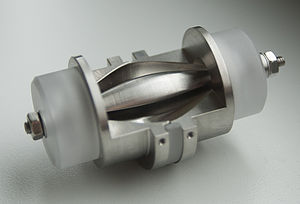
\includegraphics[width=0.5\textwidth]{iontrap}
	\caption{Kingdon离子肼}
	\label{gf:iontrap}
\end{figure}

\subsection{量子逻辑门}

最常见的量子运算架构基本组成单元就是量子逻辑门,下面将要介绍的量子计算机体系架构都基于“量子门”这一概念。在前沿的理论计算学术领域,量子计算机所用到的操作都会被形式化为“量子门”,通过这种封装的行为进行计算,使得量子理论化更加便捷,这也是学术界普遍采用的做法。量子门电路就是我们之前提到过的酉矩阵,其简单形式之一就是Hadamard矩阵。比如我们要实现一个功能,它有两个输入,一个是控制位,占1比特,另一个是数据位,占1比特,该功能的行为如下:
\begin{enumerate}
  \item 如果控制位$x=|0\rangle$,则数据位输出保持原值$y_out = y$
  \item  否则,数据输出位取反,$y_{out} = ! y$
\end{enumerate}
这种逻辑用量子门实现的形式如下式\ref{eq:quantumgate}所示。
\begin{equation}
\label{eq:quantumgate}
Q_{gate} = \left[\begin{array}{cccc}1 & 0 & 0 & 0 \\0 & 1 & 0 & 0 \\0 & 0 & 0 & 1 \\0 & 0 & 1 & 0\end{array}\right]
\end{equation}
这种逻辑门形式就可以达成上述所需的功能。以矩阵化的量子操作来构造逻辑门其实十分便捷,我们可以基于这些基本的规则构造任意传统电路的逻辑门,除此外我们也能构造更复杂的逻辑门,或者将简单的逻辑门基于量子特性达成复杂特性,关于Hadamard矩阵更深的用法将在后文中进一步涉及。

\subsection{基于量子门与叠加态特性的典型算法}

一个比较典型的算法是Deutsch算法在量子架构下的实现。Deutsch算法主要解决这样一个问题:给定一个函数$f : \{0,1\} \rightarrow \{0,1\}$,如果$f(0) \ne f(1)$则该函数是“异函数”,如果$f(x)=f(y)$则称该函数为“同函数”。Deutsch算法的主要解决的问题就是,给定一个函数,不允许观察函数的实现过程与内部结构,只能将函数作为一个黑盒看待,而我们能做的就是对该函数进行任意次的输入(可以自行选择输入任何合法的值)并观察此函数的输出,我们要通过某种方法测试该函数,并最终给出结论:“该函数是异函数还是同函数”。

对于普通计算机能支持的过程而言,唯一可行的思路就是遍历输入该函数的整个定义域,直到发现输出了不同的值,由此判定为异函数,或者完全遍历完成,发现所有输出都相等,由此判定为同函数。这样做费时费力,而且问题的规模随着函数复杂度的增加、函数调用开销的增大而显著增大。此时量子计算就能够发挥功用。

在用量子算法处理这个问题之前,我们首先要稍加改造这个过程的表示形式,以适配量子运算的特性,我们构造出一个单元$U_f$,接收两个输入$|x\rangle,|y\rangle$,给出的输出是$|x\rangle,y|\oplus f(x)\rangle$,这样做的目的是使得这个单元服从酉矩阵对可反演性的要求。

我们借助于之前提到过的Hadamard矩阵$H$,将输入$|0\rangle,|1\rangle$作为原始输入进行预处理后再输入上述单元$U_f$,预处理令
\begin{eqnarray}
x &=& H \cdot |0\rangle = H \cdot \left[\begin{array}{c}1 \\0\end{array}\right]=\frac{|0\rangle + |1\rangle}{\sqrt{2}} \\
y & = & H \cdot |1\rangle = H \cdot \left[\begin{array}{c}0 \\1\end{array}\right]=\frac{|0\rangle - |1\rangle}{\sqrt{2}}
\end{eqnarray}

经过$U_f$单元运算后,得到结果如下式\ref{eq:xout1}、\ref{eq:yout1}所示
\begin{eqnarray}
\label{eq:xout1}
x' & = & \frac{(-1)^{f(0)|0\rangle} + (-1)^{f(1)|1\rangle}}{\sqrt{2}} \\
\label{eq:yout1}
y' & = &  \frac{|0\rangle - |1\rangle}{\sqrt{2}}\\
\label{eq:xout2}
x_{out} &=& \begin{cases}
    (\pm 1) | 0\rangle  &  \text{同函数}, \\
    (\pm 1) | 1\rangle  &  \text{异函数}.
	\end{cases} \\
\label{eq:yout2}
y_{out} &=& y' = \frac{|0\rangle - |1\rangle}{\sqrt{2}}
\end{eqnarray}

当使得$x'$再次经过$H$处理一次并保持$y'$不变后,会得到如式\ref{eq:xout2}、\ref{eq:yout2}所示,此时只需观察x即可通过仅调用$f$一次得知函数的异同性了。


\subsection{MUSIQC架构}

对于数据的传输,通常认为较经典的是QLA传输架构\cite{qla},但这些旧有的架构很多是早期实验性尝试的产物,常常有反应速度慢、可扩展性差、容纳qubits数量极少等通病。近期,在旧有架构的基础上,出现了一些新型的有代表性的运算、存储、传输架构,比如其中较新的MUSIQC架构\cite{largeq}(modular universal scalable ion trap quantum-computer),有效的可控量子比特数目可达$10^{6}$个,读写操作缩短到$10\mu$s级。该架构中计算机的读写形式如下图\ref{gf:qubit_read}所示。

\begin{figure}[H]
	\centering
	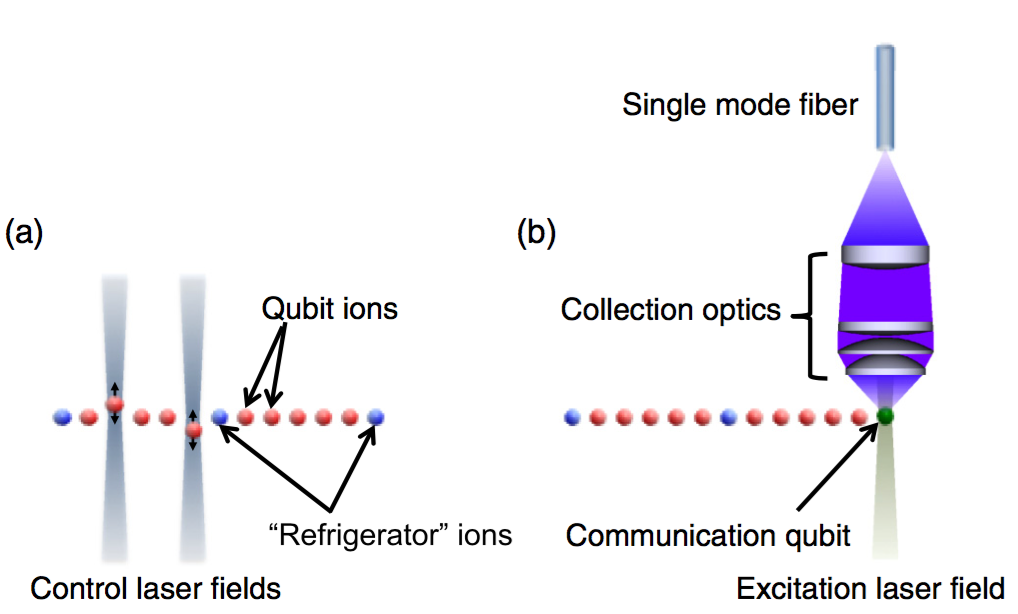
\includegraphics[width=0.5\textwidth]{qubit_read}
	\caption{线性读写,(a)中红色为存储单元,蓝色为分隔单元,用来防止溢出干扰(crosstalk)。(b)中表示的是电子干涉光子,使得光子携带相同信息,传输到光纤中。}
	\label{gf:qubit_read}
\end{figure}

在进行信息转移时,有两种模型可以使用,如下图\ref{gf:interfere}所示。

\begin{figure}[H]
	\centering
	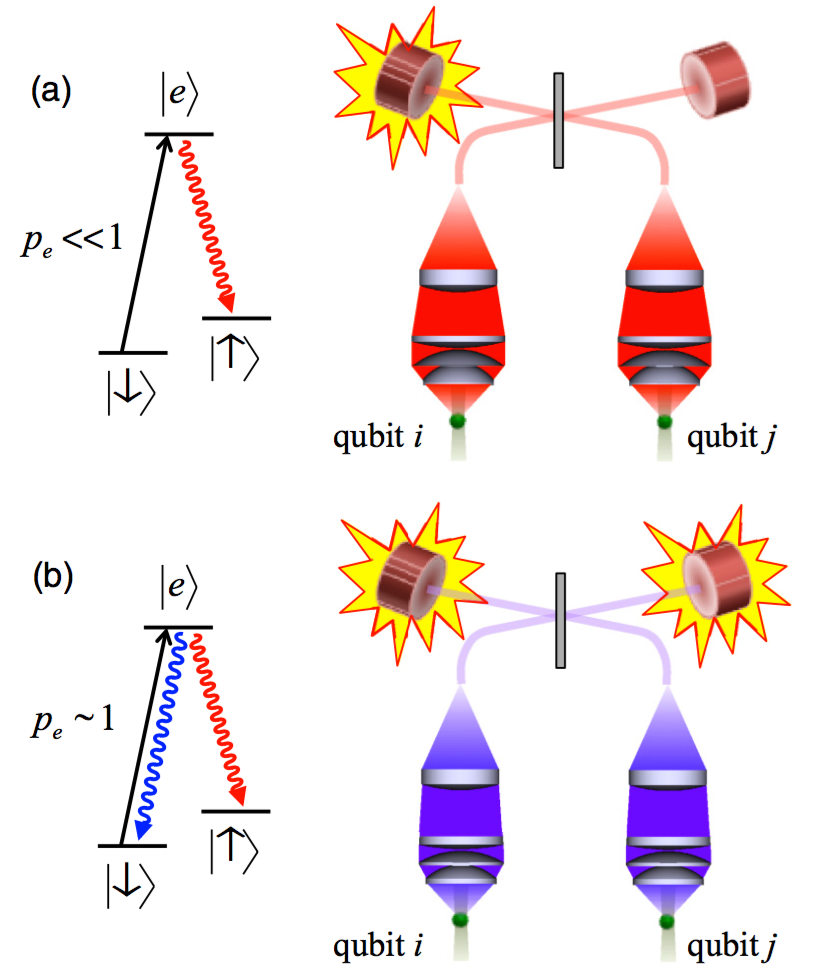
\includegraphics[width=0.5\textwidth]{interfere}
	\caption{干涉同步}
	\label{gf:interfere}
\end{figure}

对于(a)类干涉,其特点是将$i,j$两个比特作等量叠加。在任一光子接收器上接收到信号,即代表量子纠缠成功,结果即如式\ref{eq:eulersuperpos}。对(b)类干涉,其特点是纠缠结果与光子频率$\nu$有关,会影响叠加的权重。当系统是全对称时,两种方法是等价的。

在任意情况下,干涉过程成功所占用的平均时间都可表达为$\tau_{E}=1/(R_{p})$\cite{largeq},其中R是初始化过程重复率,p是纠缠成功概率。一般来说,第一种存储方式耗时约为$\tau_{E} \sim 5ms$,第二种耗时约$\tau_{E} \sim 250ms$。束缚粒子的量子存储与运算单元(下称ELU)之间通过光纤通讯,一般采用集中式架构,这种架构中的通信以一种路由的形式进行,所有光纤都连接到一个光纤交换机上(OXC optical crossconnect)由交换机负责维护数据模型。

上述信息交换是基于SPDC(Spontaneous parametric down-conversion)量子纠缠法\cite{spdc}。该方法使用非线性晶体作为分射镜,将一束光子分为两个,如果分出的两束光有相同的相位,则为I型纠缠,若两束光相位相互正交,则为II型纠缠。产生纠缠的过程如图\ref{gf:spdc}所示。

\begin{figure}
\begin{center}
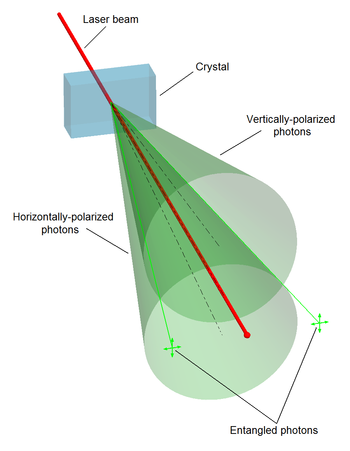
\includegraphics[width=4in]{spdc}
\caption{SPDC光量子纠缠}
\label{gf:spdc}
\end{center}
\end{figure}

如上文所述,该架构的运算方式同样基于不同振幅、相位的激光照射,加入了OXC并实现了I型、II型纠缠之后,该模型的传输速度与运算速度都具有相当的优势,如图\ref{gf:musiqc}所示。但同时该计算机体系结构也有相应的不足,由于目前量子传输技术的限制与将运算指令集映射为矩阵变换的数学研究尚且不足,MUSIQC架构的计算机与其前一代量子运算架构一样,都暂未能成为指令型计算机,对该架构量子计算机的编程都仍以硬件堆画形式进行。

\begin{figure}
\begin{center}
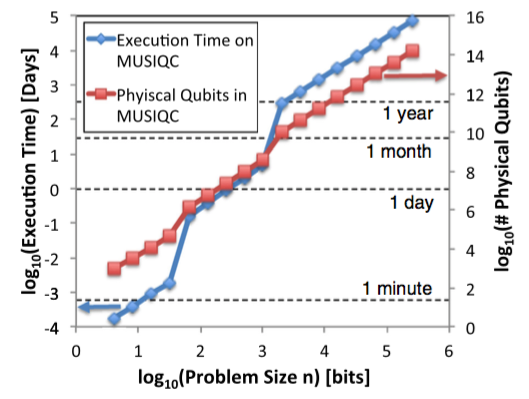
\includegraphics[width=2.5in]{musiqc_performance}
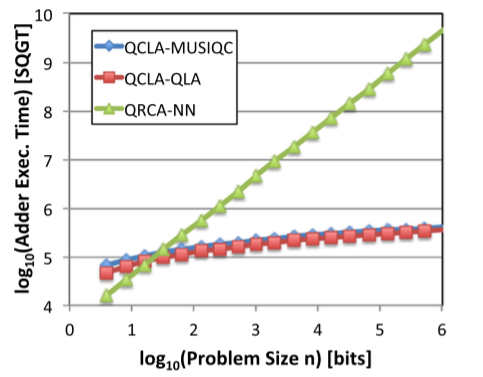
\includegraphics[width=2.5in]{musiqc_time}
\caption{效能对比}
\label{gf:musiqc}
\end{center}
\end{figure}

\subsection{量子元胞自动机}

量子元胞自动机又称QCA(Quantum Cellular Automata),这是一种基于自动机的抽象运算模型,概念完全源于冯诺伊曼的自动机范式。基于量子技术的自动机系统相比传统CMOS有速度快、耗电极低的优势\cite{qca}。

量子元胞自动机的主要构成如下。

\begin{enumerate}
  \item 每个元胞都是同构的、有限维量子系统;
  \item 每个元胞都与周围元胞邻接,形成有界或无界的邻接网络;
  \item 递推过程具有对称性,其中之一局域性是指每个元胞都只与周围元胞状态有关,其二同质性是指这种递推是广泛共同发生与网络上的;
  \item 元胞状态空间的定义、可能的操作都是基于量子的特性构造的。
\end{enumerate}

另一个重要特性是量子元胞自动机须能担任通用计算的要求,能够利用量子机制模拟图灵机行为,能够规划任意量子电路或模仿任意其他自动机。

近期提出的量子元胞机具有一些更细致的特性与要求。这种要求是基于量子运算的物理封闭性提出的。该特性基于量子矩阵运算可逆的特性,指出量子元胞自动机在明确递推策略的前提下是可逆自动机,执行的操作也是可逆的线性变换。

\subsection{流水线量子计算机架构}

相比于实际的计算机体系结构工程要求,上述QCA更偏重于概念支持,于是之后有人提出了更加工程化偏重实质的Quantum-dot Cellular Automata(虽然该架构因为其较大的贡献与影响,被看作QCA的升级版与接班人,因而有时直接被人称为QCA,但这里为了明确概念,下文将称它为QdCA),QdCA架构在QCA的基础上做了很多优化与落实方案的探究。相比VLSI和CMOS,这种架构铺展面积小、布线紧凑、能耗低的特性使得其成为微处理器与嵌入式处理器的一个非常有潜力的发展方向。

为了进一步达成效能优化,同时也为了为了解决一些QdCA存在问题,近期一种基于QdCA并结合流水线的量子计算架构被提出\cite{pipeline}。

总的来说,该方案是在尝试解决高速运算Hadamard变换(DHT)的过程中被提出的。为了提高速度,该方案采用了全并行的计算架构并实现了支持多比特加法的QdCA。进一步地,该架构采用了位序列流水线架构来在QdCA结构上计算DHT问题。同时,该架构采用了只需要六个门和1个流水限阀的1位加减单元,这里采用的流水限阀工作时只需要1位逻辑门位和极少的布线支持即可快速完成运算。在采用了这些措施后,整体架构的延时下降了74\% ,若进行全并行运算(比如运行字长4或8的算法),则可充分利用流水线降低91\%的延迟。

首先我们给出Hadamard变换的定义,$N\times N$的Hadamard矩阵定义为$H_N=H_{N/2}\otimes H_{2}=H_{2} \otimes H_{N/2}$,其生成子$H_2$如下式\ref{eq:h2}所示。
\begin{eqnarray}
\label{eq:h2}
H_2 & = & \left[\begin{array}{cc}1 & 1 \\1 & -1\end{array}\right] \\
\label{eq:hn}
H_N & = & \left[\begin{array}{cc}H_{N/2} & H_{N/2} \\H_{N/2} & -H_{N/2} \end{array}\right] 
\end{eqnarray}
要求得的H变换结果如下式\ref{eq:DHT}所示。
\begin{eqnarray}
X&=&{X(n),n=1,2,3,...,N-1} \\
\label{eq:DHT}
Y(k)&=&\sum_{n=0}^{N-1}H_{N}(k,n)X(n) \\
\end{eqnarray}
for $0 \le k \le N-1$。
更加形式化地,可将该操作视为下式。
\begin{eqnarray}
 \left[\begin{array}{c}Y_0 \\Y_1 \\Y_2 \\Y_3\end{array}\right] & = & H_4 \cdot  \left[\begin{array}{c}X_0 \\X_1 \\X_2 \\X_3\end{array}\right] \\
\label{eq:y0}
Y_0 & = & (X_0 + X_2) + (X_1 + X_3) \\
\label{eq:y1}
Y_1 & = & (X_0 + X_2) - (X_1 + X_3) 
\end{eqnarray}

对于式\ref{eq:y0} 、\ref{eq:y1} 如果采用全并行策略则$X_0 \pm X_2$就需要用全并行加减器来做。该架构引入了Pudi等人提出的加减元件\cite{adder},应用此元件制成的长度$W=4$的电路见图\ref{gf:qcaw4} , 长度为8的电路见图\ref{gf:qcaw4}。 

\begin{figure}[H]
\begin{center}
\includegraphics[width=4in]{qcaw=4}
\caption{基于QdCA的4位宽加减法电路结构}
\label{gf:qcaw4}
\end{center}
\end{figure}

\begin{figure}[H]
\begin{center}
\includegraphics[width=4in]{qcaw=8}
\caption{基于QdCA的8位宽加减法电路结构}
\label{gf:qcaw8}
\end{center}
\end{figure}
为了挖掘该架构下并行的能力,如果用c来表示进位(Carry)的话,我们可将$Y$	进一步细化到位的粒度,如下式\ref{eq:y0bit}所示。
\begin{equation}
\label{eq:y0bit}
Y_0=(x_{0,i} + x_{2,i} + c_{0,i}) + (x_{1,i} + x_{3,i} + c_{1,i})
\end{equation}
根据对并行的需要,最终4位加减器的架构如图\ref{gf:addsub}所示。在该体系结构中,尝试解决hadamard变换问题的过程如下
\begin{figure}[H]
\begin{center}
\includegraphics[width=4in]{addsub}
\caption{4位全并行加减器}
\label{gf:addsub}
\end{center}
\end{figure}

这种设计是位流水的,也就是说改加法器会每个时钟产生一个结果,依次为$Y_0 , Y_1 ,Y_2 ,Y_3$。因为对于8位数加减最多需要输出10位,因此相应地8位加法器所需时钟周期为10个。该架构(图\ref{gf:addsub}所示)的主要特点是流水线一位加法器,与带反馈的流水线限阀。该架构的性能情况如图\ref{gf:qca_performance}所示。

\begin{figure}[H]
\begin{center}
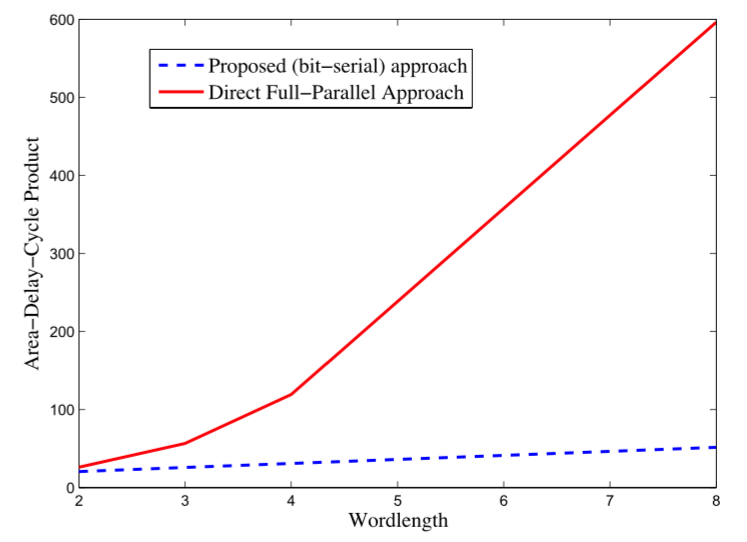
\includegraphics[width=4in]{qca_performance}
\caption{性能对比}
\label{gf:qca_performance}
\end{center}
\end{figure}

性能对比图表\ref{gf:qca_performance}主要对比了流水线QdCA量子计算架构与传统基于QCA全并行加法器的架构的性能关系,并对解决类似傅立叶变换问题这样高度可并行的计算问题时的测试效果进行了验证。图中所示的ADC是指架构实现的面积、延迟与时钟滴答的乘积指标。这种评估方式比传统的面积-延迟乘积方式更加适合于公平地评估与比较串行与并行之间的效率异同。由图标可看出,该架构的运算电路ADC只是全并行电路的26\% 。当$W=8$时更是达到了9\% ,优势比较显著。

\newpage
\section{结论}
量子计算架构作为一个极为有趣、有前景的计算方式,极大利用了从物理过程中发掘出来的可计算性,使得多种叠加态同步地接受相同操作,经过合理设计的运算可以使得不符合要求的结果成为相互法向的状态而彼此抵消,并使得正确的答案形成的状态彼此加强,最后输出,这是一种代价极低的真正的并行方法,如果能深入探究并合理地利用,将会对新一代计算的需求产生重大贡献,如果未来产生的新方案能够采用类似传统计算机基于cache的细化设计\cite{cache},或挖掘酉矩阵算符的表达能力制作出具有指令集(RISC或CISC)的微型通用芯片(这里还有很多工作需要思考\cite{risccisc}),还有对多量子核共用存储的模式借助经典架构的锁\cite{lock}进行管理,同时加入一些被证明有巨大提升的辅助架构,比如经典架构中的预测和投机调度\cite{schedule},借助经典微内核研发中的经验\cite{microkernel20years},量子计算架构将会迸发出更强大的能力。

然而与此同时,相关领域也出现了一些显著问题。量子计算机的物理概念大约在2000年前后成型,并在2005-2012年间持续发酵,成为一个大家关注的热点,相关重量级的论文也相继在顶级期刊会议上发表。之后到2015-2016年量子计算机话题逐步进入平缓期,2015年前后在顶级期刊会议发表的量子计算机体系结构论文大幅减少,精品论文只有寥寥可数的几篇,2017年尚未见到任何量子计算架构论文在顶会发表。这说明物理发现的红利正在退去,在没有更新的物理成果支持出现前,量子计算是否能保持其领先的架构概念,尽快落实应用,目前来看,仍还需要更多研究才可获知。


\newpage
\bibliography{refs}
\bibliographystyle{unsrt}
\end{document}  





